\documentclass{beamer}
\usetheme{Warsaw}
\usepackage{polski}
\usepackage[utf8]{inputenc}

\title{Kształtowanie pola elektromagnetycznzego za pomocą elementów podfalowych}
\subtitle{Autoreferat}
\author{Marcin Stolarek}
\institute{Zakład Optyki Informacyjnej, Wydział Fizyki UW}
\date{\today}

\begin{document}

\frame{\titlepage}

\frame{\tableofcontents}

\section{Wielowarstwy metaliczno-dielektryczne}
\subsection{Pryzmat do obrazowania podfalowego}
\begin{frame}
	\begin{columns}
		\begin{column}{0.5\textwidth}
			\begin{figure}
				\includegraphics[width=\textwidth]{../images/multilayer/prism.png}
			\end{figure}
		\end{column}
		\begin{column}{0.5\textwidth}
		\end{column}
	\end{columns}
		
\end{frame}

\begin{frame}[t]
	\begin{columns}
		\begin{column}{0.5\textwidth}
			\begin{figure}
				\includegraphics[width=\textwidth]{../images/multilayer/prism04.png} \\
				\includegraphics[width=\textwidth]{../images/multilayer/prism08.png} \\
			\end{figure}
		\end{column}
		\begin{column}{0.5\textwidth}
				\includegraphics[width=\textwidth]{../images/multilayer/prism12.png}\\
				Wydajność i FWHM wiązki wychodzącej zależą nie tylko od kąta łamiącego pryzmatu, ale i od przesunięcia wiązki wchodzącej, wskazując na brak możliwości stosowania modelu ośrodka efektywnego we wszystkich tego typu układach.
		\end{column}
	\end{columns}
		
\end{frame}

\subsection{Projektownie układów przez ray tracing}

\begin{frame}
	\begin{columns}
		\begin{column}{0.5\textwidth}
			\begin{figure}
				\includegraphics[angle=90,width=\textwidth]{../images/multilayer/konc_eps_mgr.png}\\
				\includegraphics[angle=90,width=\textwidth]{../images/multilayer/konc_ene_mgr.png}
			\end{figure}
		\end{column}
		\begin{column}{0.5\textwidth}
			\begin{itemize}
				\item Inżynierski model projektowania.
				\item Ograniczony silną dyfrakcją poza strukturą.
				\item Ścisłe modelowanie niezbędne.
			\end{itemize}
		
		\end{column}
	\end{columns}
		
\end{frame}

\begin{frame}
	\begin{columns}
		\begin{column}{0.5\textwidth}
			\begin{figure}
				\includegraphics[width=\textwidth]{../images/multilayer/konc_polk_poynt.png}\\
			\end{figure}
		\end{column}
		\begin{column}{0.5\textwidth}
				\includegraphics[width=\textwidth]{../images/multilayer/konc_coreshell_energy.png}\\
		\end{column}
	\end{columns}
		
\end{frame}


\subsection{Wpływ gładkości warstw}


\section{Siatki metalowe do kształtowania fali w THz}
\subsection{Antena dla detektora THz}
\begin{frame}
	\begin{columns}
		\begin{column}{0.5\textwidth}
			\begin{figure}
				\includegraphics[width=\textwidth]{../images/antenaThz/schemat.png}\\
				\includegraphics[width=\textwidth]{../images/antenaThz/rezonant_trans_f001.png}\\
			\end{figure}
		\end{column}
		\begin{column}{0.5\textwidth}
			\begin{figure}
				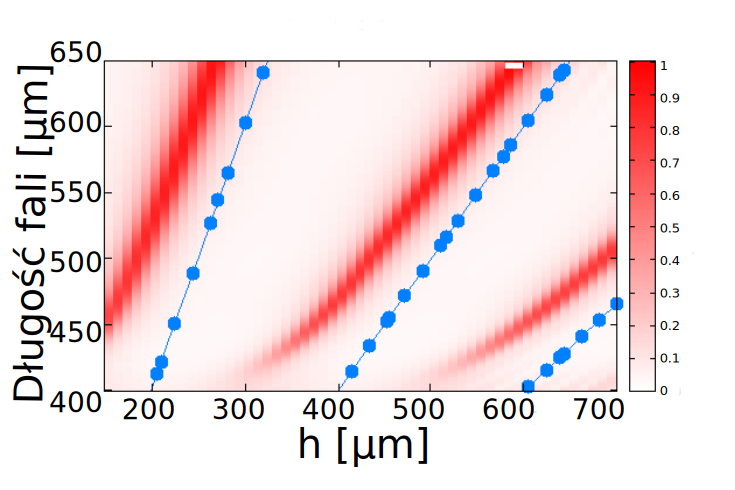
\includegraphics[width=\textwidth]{../images/antenaThz/rezonant_trans_f01.png}\\
				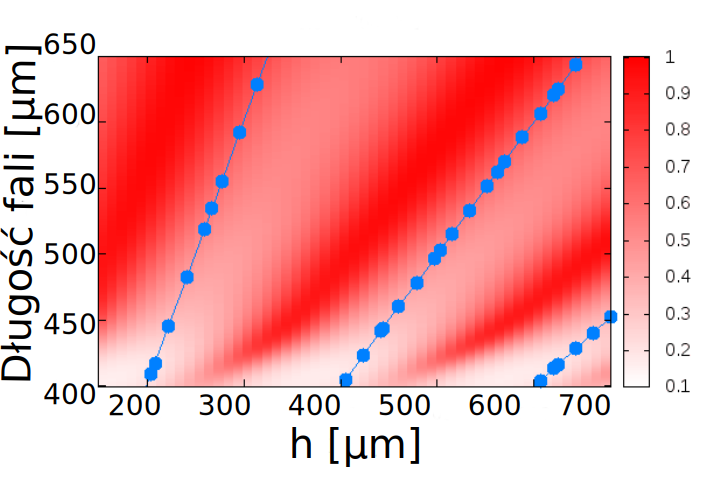
\includegraphics[width=\textwidth]{../images/antenaThz/rezonant_trans_f05.png}\\
			\end{figure}
		\end{column}
	\end{columns}
		
\end{frame}

\subsection{Podwójne metalowe siatki dyfrakcyjne}
\begin{frame}
	\begin{columns}
		\begin{column}{0.5\textwidth}
			\begin{figure}
				\includegraphics[width=\textwidth]{../images/dmg/letters_eneden.png}
			\end{figure}
		\end{column}
		\begin{column}{0.5\textwidth}
			\begin{figure}
				\includegraphics[width=\textwidth]{../images/dmg/letters_schemat.png}
			\end{figure}
		\end{column}
	\end{columns}
		
\end{frame}

\begin{frame}
	\begin{columns}
		\begin{column}{0.5\textwidth}
			\begin{figure}
				\includegraphics[width=\textwidth]{../images/dmg/letters_exp_setup.png}\\
				\includegraphics[width=\textwidth]{../images/dmg/letters_spect.png}\\
			\end{figure}
		\end{column}
		\begin{column}{0.5\textwidth}
				\includegraphics[width=\textwidth]{../images/dmg/letters_exp.png}\\
		\end{column}
	\end{columns}
		
\end{frame}

\begin{frame}
	\frametitle{Podniesienie kontrastu}
	\begin{columns}
		\begin{column}{0.5\textwidth}
			\begin{figure}
				\includegraphics[width=\textwidth]{../images/dmg/kontrast_schemat.png}\\
				\includegraphics[width=\textwidth]{../images/dmg/kontrast_maps.png}\\
			\end{figure}
		\end{column}
		\begin{column}{0.5\textwidth}
			\begin{figure}
				\includegraphics[width=\textwidth]{../images/dmg/kontrast_energy.png}\\
			\end{figure}
		\end{column}
	\end{columns}
		
\end{frame}

\begin{frame}
	\frametitle{Polaryzacja radialna}
	\begin{columns}
		\begin{column}{0.5\textwidth}
			\begin{figure}
				\includegraphics[width=\textwidth]{../images/dmg/express_exp_setu.png}\\
			\end{figure}
		\end{column}
		\begin{column}{0.5\textwidth}
			\begin{figure}
				\includegraphics[width=\textwidth]{../images/dmg/express_siatki.png}\\
			\end{figure}
		\end{column}
	\end{columns}
		
\end{frame}

\begin{frame}
	Struktura zaprojektowana do:
	\begin{figure}
		\includegraphics[width=\textwidth]{../images/dmg/express_high_contrast.png}\\
	\end{figure}
	Eksperyment wykonany w "przeciwnym" kierunku:
	\begin{figure}
		\includegraphics[width=\textwidth]{../images/dmg/express_zarmata.png}\\
	\end{figure}
		
\end{frame}




\section{Realizacja PML przy pomocy wielowarstw}
\begin{frame}
	\begin{figure}
				\includegraphics[width=\textwidth]{../images/pml/oqe_schemat.png}
			\end{figure}

	\begin{columns}
		\begin{column}{0.5\textwidth}

		\end{column}
		\begin{column}{0.5\textwidth}

		\end{column}
	\end{columns}
		
\end{frame}

\begin{frame}
	\begin{figure}
				\includegraphics[width=\textwidth]{../images/pml/oqe_materials.png}
	\end{figure}
		
\end{frame}


\begin{frame} [t]
	\begin{columns}
		\begin{column}{0.5\textwidth}
			\begin{figure}
						\includegraphics[width=\textwidth]{../images/pml/oqe_materials.png}
			\end{figure}
			Realizacja materiałw z  $\mu \ne 1$ lub wzmocnieniem nie jest możliwa, konieczne jest przybliżenie propnowanego PML realnymi materiałami.			
		\end{column}
		\begin{column}{0.6\textwidth}
			\begin{figure}
						\includegraphics[width=0.9\textwidth]{../images/pml/oqe_reflection_kat.png}\\
			\end{figure}
				
		{\tiny	Dzięki oddzielnemu rozważaniu polaryzacji możemy wykluczyć zależność od części parametrów materiałowych. Nie możemy jednak wykluczyć zespolonego charakteru $\mu$.}

			\begin{figure}
						\includegraphics[width=0.9\textwidth]{../images/pml/oqe_reflection_kat_simp.png}
			\end{figure}

		\end{column}

	\end{columns}
		
\end{frame}


\begin{frame}
	\begin{columns}
			\begin{column}{0.5\textwidth}
			\begin{figure}
						\includegraphics[width=\textwidth]{../images/pml/oqe_trans_refl.png}
			\end{figure}
		\end{column}
		\begin{column}{0.5\textwidth}
			\begin{figure}
						\includegraphics[width=1.1\textwidth]{../images/pml/oqe_coreshell.png}
			\end{figure}
		\end{column}

	\end{columns}
		
\end{frame}





\begin{frame}
\frametitle{Title}
Lorem ipsum dolor sit amet, consectetur adipisicing elit, sed do eiusmod tempor incididunt ut labore et dolore magna aliqua.
\end{frame}

\end{document}



%% Kawalki do przeklejania:
%% Ramka z kolumnami i obrazkiem:
\begin{frame}
	\begin{columns}
		\begin{column}{0.5\textwidth}
			\begin{figure}
				\includegraphics[width=\textwidth]{../images/pml/}
			\end{figure}
		\end{column}
		\begin{column}{0.5\textwidth}
		asd
		\end{column}
	\end{columns}
		
\end{frame}


